% English article version of the BIL482 project. Compile with pdfLaTeX (e.g. on Overleaf).
\documentclass[conference,a4paper]{IEEEtran}
\usepackage[T1]{fontenc}
\usepackage[utf8]{inputenc}
\usepackage{graphicx}
\usepackage{booktabs}
\usepackage{amsmath,amssymb}
\usepackage[hidelinks]{hyperref}
\usepackage{cite}
\graphicspath{{figures/en/}}

\begin{document}

\title{How Well Do Turkish Hallucination Detectors Work?\\ A Single-Protocol Benchmark, a Stronger Detector,\\ and a Native Turkish Test Set}

\author{\IEEEauthorblockN{İshak Türk}
\IEEEauthorblockA{BIL482 Term Project (student no. 23120205003)\\
Code and data: \url{https://github.com/ishakturk/Turkish-RAG-Hallucination-Detector}}}

\maketitle

\begin{abstract}
Retrieval-augmented generation (RAG) systems still produce statements their context does not support. Small encoder models that tag unsupported answer spans are a cheap and fast defence, and several have been released for Turkish, all trained and tested on a machine translation of RAGTruth. We re-evaluate all seven existing Turkish detectors and two classical baselines under one reproducible protocol: character-level scoring shared by every tokenizer, per-system thresholds tuned on a held-out dev split, source-grouped bootstrap intervals, and a final test opened once under a pre-registered analysis plan. Our final model, mmBERT-base fine-tuned on the cleaned data with a class-weighted loss, beats the pre-registered best baseline by $+0.070$ example F1 [0.049, 0.093] and $+0.100$ span F1 [0.075, 0.125], and every existing detector in exploratory comparisons. Controlled runs attribute most of the gain to the multilingual base model; hallucination pretraining and native-data augmentation do not help on the translated test. We then build a native Turkish test set of 184 answers written by Qwen3-8B and DeepSeek over Wikipedia and legal contexts. Every supervised detector loses most of its recall there (our final model: example F1 $0.766 \rightarrow 0.458$), while the model trained with native Turkish augmentation is best (0.592). Translated benchmarks overstate how well Turkish detectors work.
\end{abstract}

\begin{IEEEkeywords}
hallucination detection, retrieval-augmented generation, Turkish NLP, span detection, evaluation
\end{IEEEkeywords}

\section{Introduction}
A RAG answer is \emph{faithful} when every statement is supported by the retrieved context. We call any unsupported statement a hallucination, even if it happens to be true in the world. Encoder-based detectors such as LettuceDetect~\cite{kovacs2025lettucedetect} frame this as token classification over \texttt{[CLS] prompt [SEP] answer [SEP]} and run in milliseconds. For Turkish, Turk-LettuceDetect~\cite{tas2025turk} translated RAGTruth~\cite{niu2024ragtruth} with an LLM (RAGTruth-TR) and released several detectors.

Three gaps motivated this work:
\begin{itemize}
\item Prior Turkish results are reported at mixed and partly unlabeled levels, and the evaluation code is not public. In the paper's results table, AUROC equals recall in all twelve rows.
\item No validation split is described for model selection or thresholds.
\item Everything is measured on translated text.
\end{itemize}

We contribute:
\begin{enumerate}
\item a single-protocol, reproducible benchmark of all Turkish detectors;
\item a detector that wins the pre-registered primary comparison;
\item controlled answers on base model, warm start, recipe and augmentation;
\item a native Turkish test set (184 answers, LLM-labeled, human-validated) that measures the translated-to-native gap.
\end{enumerate}

\section{Related Work}
RAGTruth~\cite{niu2024ragtruth} is the standard span-labeled corpus (QA, data-to-text, summarization). Encoder detectors include LettuceDetect (ModernBERT~\cite{warner2024modernbert}), Luna~\cite{belyi2025luna} and RAG-HAT~\cite{song2024raghat}. Further work uses attention features~\cite{ogasa2025multiview} and temporal signals~\cite{itkin2026temporal}. Generative span detectors trained with reinforcement learning (RL4HS~\cite{su2025rl4hs}, SOPO~\cite{dong2026sopo}) and broader grounding settings~\cite{kovacs2026beyond} are stronger but far larger. SOPO reports LettuceDetect-Large at 58.9 span-level F1, against 79.22 example-level F1 in its own paper: levels must not be mixed. Multilingual resources with Turkish (HalluVerse25~\cite{abdaljalil2025halluverse25}, HalluVerse-M3~\cite{abdaljalil2026halluversem3}) lack context-grounded spans, and MultiWikiQHalluA~\cite{thoresen2026multiwiki} has no Turkish split. Candidate base encoders are TabiBERT~\cite{turker2025tabibert} (Turkish-native), mmBERT~\cite{marone2025mmbert}, EuroBERT~\cite{boizard2025eurobert} and Ettin~\cite{weller2025ettin}. RAGTurk~\cite{kose2026ragturk} studies Turkish RAG pipelines.

\section{Data}
\textbf{RAGTruth-TR} has 17,790 responses (2,965 sources $\times$ 6), with no source id and no validation split. We recovered source ids by aligning rows to the English RAGTruth in file order (99.99\% pass three checks: span count, digits and length ratio). A rule-based audit dropped 1.06\% of rows (spans out of bounds, span-count mismatch with English, repetition, truncation). It also found that translation added an unlabeled number to 3.5\% of answers.

\textbf{Splits.} The official test set was split once by source into a dev set (540 responses) for every threshold and selection decision, and a final test (2,160 responses), scored once. 5\% of train sources form a validation set for early stopping.

\textbf{Augmentation.} From Turkish Wikipedia QA (\texttt{multi-wiki-qa}, \texttt{tr}) DeepSeek wrote a faithful answer or summary per context, and for half of them a version with tagged errors. We found and removed a position shortcut: in the first prompt, a third of the error spans were an appended final sentence; after the fix this fell to 3.4\% (RAGTruth-TR: 11\%). The run produced 5,484 records (33\% hallucinated) for \$0.80. Only R4 uses them.

\textbf{Native test set.} 139 Wikipedia contexts (articles disjoint from the augmentation) and 45 Turkish legal contexts were used. Half of the questions are original; half were rewritten so that the context answers them only in part, and all 203 rewrites were reviewed by hand (30 rejected). Answers come from Qwen3-8B~\cite{yang2025qwen3} and DeepSeek with the RAGTruth-TR prompt template; bare refusals were discarded. The labeling guide was written before any answer existed. Reference labels combine two independent LLM label sets ($\kappa = 0.91$ between them, 6 disagreements adjudicated by the author). The author then labeled a stratified blind sample of 50 rows without AI help:
\begin{itemize}
\item 85.7\% raw agreement, $\kappa = 0.38$ [$-0.07$, 0.73], PABAK 0.71, with only 6--7 positives in 49 rows;
\item on review, 6 of the 7 disagreements were resolved in favor of the LLM label (subtle unsupported inferences missed by the human, or omissions the guide does not count).
\end{itemize}
The final set has 47 hallucinated answers out of 184, with 52 gold spans. Hallucination is concentrated in Qwen answers (44\% vs.\ 4\% for DeepSeek) and in partly answerable questions (45\% vs.\ 9\%; Fig.~\ref{fig:rates}).

\begin{figure*}[t]
\centering
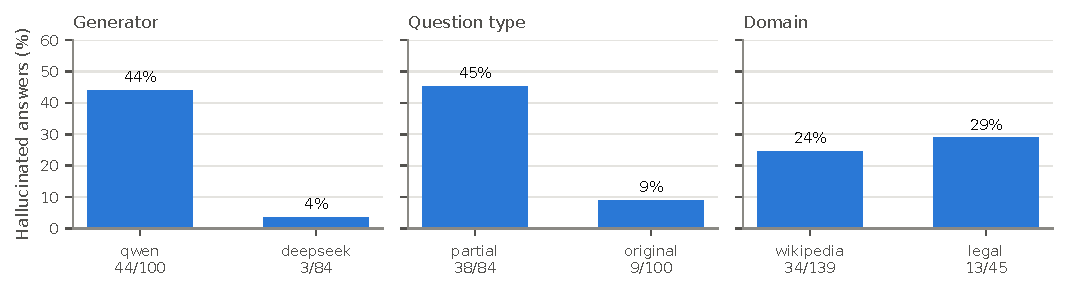
\includegraphics[width=\textwidth]{fig7_native_rates.pdf}
\caption{Share of hallucinated answers in the native Turkish test set.}
\label{fig:rates}
\end{figure*}

\section{Method}
\textbf{Scoring across tokenizers.} Every model outputs a probability per answer \emph{character} (each token's probability is spread over its characters). A word is flagged when its maximum character probability reaches $\tau$; Turkish suffixes after an apostrophe stay with their stem. Close flagged words merge into spans. Example F1 asks whether an answer has any predicted span; span F1 uses character overlap. Both are computed for the hallucinated class.

\textbf{Runs.} Each run pair differs in one factor:
\begin{itemize}
\item R0: TabiBERT with a Newmind-style recipe (6 fixed epochs, plain cross-entropy, uncleaned data, 1 seed);
\item R1: TabiBERT with our recipe (AdamW, lr $3\cdot10^{-5}$, class-weighted cross-entropy, early stopping on validation word F1, at most 4 epochs, cleaned data);
\item R2: mmBERT-base with the same recipe;
\item R3: the KR Labs v2 mmBERT hallucination detector as a warm start;
\item R4: R2 plus augmentation (25\% of training examples).
\end{itemize}
R1--R4 use 3 seeds each.

\textbf{Protocol.} Each of the 22 systems, baselines included, gets $\tau_{\text{example}}$ and $\tau_{\text{span}}$ tuned on dev; they were frozen in a commit before the test was opened. The final model (R2, by the pre-registered rule) is compared with the best dev baseline (TurkEmbed4STS-HD) using a source-grouped, seed-averaged bootstrap (2,000 replicates) and per-seed paired permutation tests (10,000 permutations).

\section{Results}
\textbf{Primary result.} R2 beats the best baseline by $+0.070$ example F1 [0.049, 0.093] and $+0.100$ span F1 [0.075, 0.125], with $p<0.001$ for every seed on both metrics (Table~\ref{tab:main}, Fig.~\ref{fig:main}). The conclusions are unchanged on the audited clean test. In exploratory paired comparisons, R2 beats all seven existing detectors on both metrics (all 14 CIs above zero). The closest are ModernBERT-tr ($+0.028$ / $+0.068$) and bge-m3 ($+0.037$ / $+0.069$).

\begin{table}[t]
\centering
\caption{Final test (2,160 responses), frozen dev thresholds. Our runs: mean over 3 seeds. CI = 95\% source-grouped bootstrap.}
\label{tab:main}
\scriptsize
\setlength{\tabcolsep}{3pt}
\begin{tabular}{@{}lccc@{}}
\toprule
System & Example F1 [CI] & Span F1 [CI] & AUROC \\
\midrule
\textbf{R2 mmBERT-base (final)} & \textbf{0.766} [0.738, 0.792] & \textbf{0.538} [0.493, 0.578] & \textbf{0.897} \\
R4 + augmentation & 0.748 [0.720, 0.774] & 0.534 [0.484, 0.573] & 0.888 \\
R3 KR Labs warm start & 0.761 [0.733, 0.785] & 0.525 [0.477, 0.570] & 0.896 \\
R1 TabiBERT & 0.716 [0.686, 0.743] & 0.487 [0.437, 0.531] & 0.870 \\
R0 Newmind recipe & 0.738 [0.705, 0.767] & 0.471 [0.417, 0.516] & 0.864 \\
\midrule
ModernBERT-tr & 0.738 [0.709, 0.765] & 0.470 [0.423, 0.510] & 0.868 \\
bge-m3 & 0.729 [0.695, 0.760] & 0.469 [0.421, 0.508] & 0.868 \\
EuroBERT-tr & 0.714 [0.679, 0.745] & 0.456 [0.402, 0.501] & 0.859 \\
TurkEmbed4STS (best dev) & 0.696 [0.661, 0.728] & 0.438 [0.395, 0.474] & 0.851 \\
Ettin-150M & 0.675 [0.642, 0.705] & 0.413 [0.367, 0.457] & 0.834 \\
Ettin-32M & 0.644 [0.608, 0.676] & 0.390 [0.329, 0.446] & 0.787 \\
KR Labs v2 zero-shot & 0.551 [0.519, 0.582] & 0.254 [0.219, 0.298] & 0.699 \\
\midrule
Word log. regression & 0.615 [0.584, 0.644] & 0.156 [0.138, 0.176] & 0.758 \\
Lexical overlap & 0.607 [0.575, 0.637] & 0.141 [0.127, 0.155] & 0.750 \\
\bottomrule
\end{tabular}
\end{table}

\begin{figure*}[t]
\centering
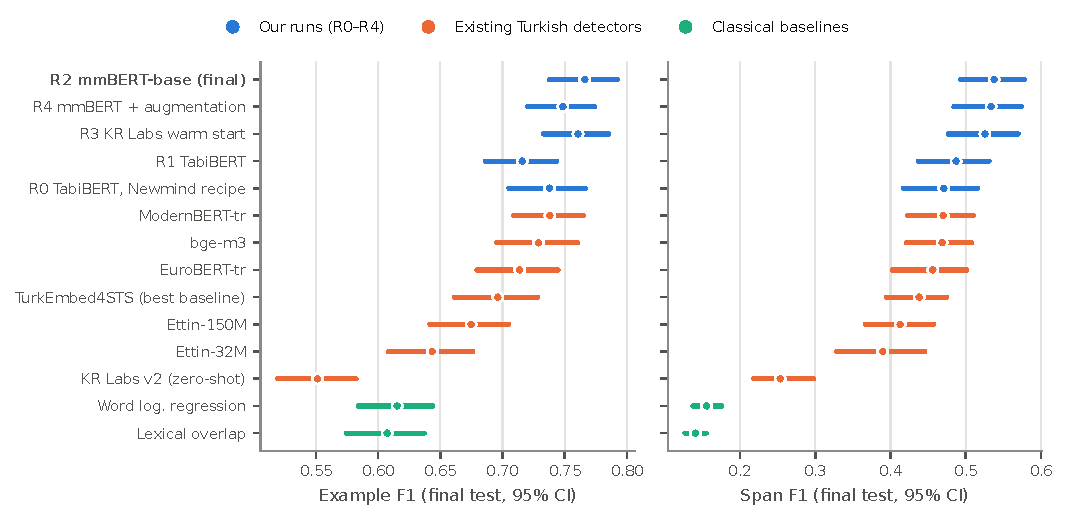
\includegraphics[width=\textwidth]{fig1_main_results.pdf}
\caption{Final-test example and span F1 with 95\% CIs.}
\label{fig:main}
\end{figure*}

\textbf{Per task.} R2 leads on QA (span F1 0.600) and data-to-text (0.574). Summarization is hard for every system (at most 0.309, reached by R4) (Fig.~\ref{fig:tasks}).

\begin{figure}[t]
\centering
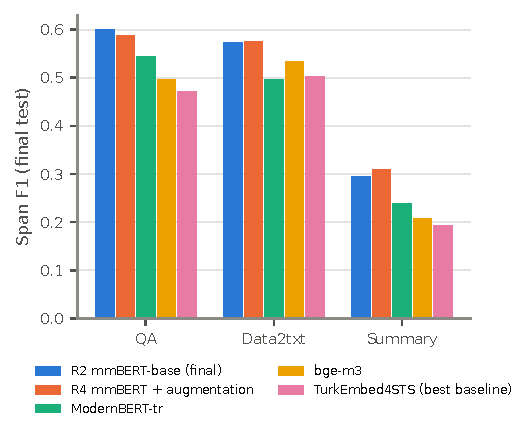
\includegraphics[width=\columnwidth]{fig3_span_f1_per_task.pdf}
\caption{Span F1 per task on the final test.}
\label{fig:tasks}
\end{figure}

\textbf{Controlled comparisons} (secondary, Fig.~\ref{fig:forest}):
\begin{itemize}
\item Q2: the multilingual base wins (R1 $-$ R2: $-0.050$ / $-0.051$, both CIs below zero), reversing a QA-only pilot.
\item Q3: hallucination pretraining does not transfer (R3 $-$ R2 CIs include zero).
\item Q4: our recipe versus the Newmind-style recipe is mixed ($-0.022$ example F1, span F1 not distinguishable). Our recipe ranks words better (word AUROC 0.897 vs.\ 0.865) and is far better on summary spans.
\item Q5: augmentation costs a little example F1 ($-0.018$) on the translated test.
\end{itemize}
Threshold tuning matters a lot. The zero-shot KR Labs model scores 0.324 example F1 at $\tau=0.5$ and 0.551 at its tuned $\tau=0.05$.

\begin{figure*}[t]
\centering
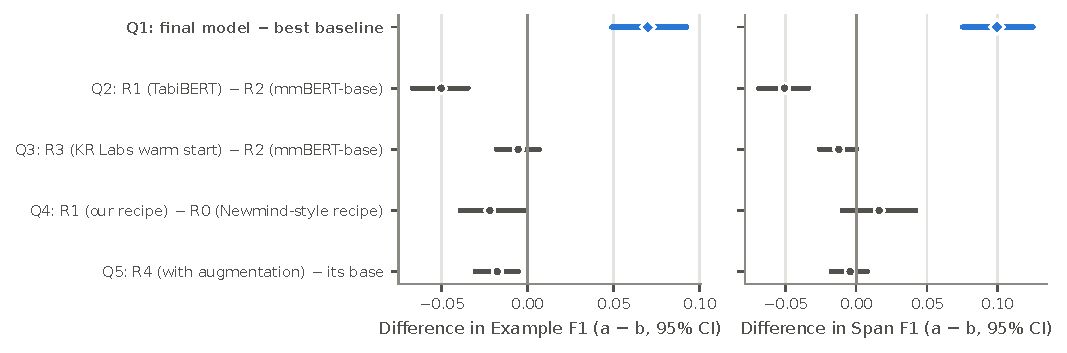
\includegraphics[width=\textwidth]{fig2_q1_q5_forest.pdf}
\caption{Pre-registered differences (a $-$ b) with 95\% CIs; only Q1 is confirmatory.}
\label{fig:forest}
\end{figure*}

\textbf{Native Turkish test} (descriptive, scored once with frozen dev thresholds; Table~\ref{tab:native}, Fig.~\ref{fig:native}).
\begin{itemize}
\item Every supervised detector drops sharply, mostly in recall. R2 has precision 0.80 but recall 0.33, and the best dev baseline falls to 0.214 example F1.
\item R4, trained with native Turkish augmentation, is best (0.592 example F1, $+0.134$ [0.037, 0.233] over R2). The gain is entirely on Wikipedia, the augmentation's source domain; on legal text the two tie.
\item The zero-shot KR Labs model has the best AUROC (0.826) but, at its frozen threshold, flags almost everything.
\item The primary comparison keeps its direction (R2 $-$ TurkEmbed4STS: $+0.244$ example F1, CI above zero).
\end{itemize}

\begin{table}[t]
\centering
\caption{Native Turkish test (184 answers, 47 hallucinated). CIs resample contexts.}
\label{tab:native}
\scriptsize
\setlength{\tabcolsep}{3pt}
\begin{tabular}{@{}lcccc@{}}
\toprule
System & Ex.\ F1 [CI] & P / R & AUROC & Span F1 \\
\midrule
\textbf{R4 + augmentation} & \textbf{0.592} [0.469, 0.696] & 0.72 / 0.51 & 0.776 & \textbf{0.361} \\
KR Labs v2 zero-shot & 0.489 [0.400, 0.573] & 0.33 / 0.94 & \textbf{0.826} & 0.307 \\
R2 (final) & 0.458 [0.321, 0.586] & 0.80 / 0.33 & 0.728 & 0.335 \\
R3 & 0.432 [0.286, 0.560] & 0.80 / 0.30 & 0.746 & 0.325 \\
R1 TabiBERT & 0.401 [0.254, 0.534] & 0.80 / 0.27 & 0.698 & 0.299 \\
EuroBERT-tr & 0.400 [0.222, 0.545] & 0.92 / 0.26 & 0.707 & 0.298 \\
R0 & 0.375 [0.215, 0.525] & 0.71 / 0.26 & 0.670 & 0.182 \\
bge-m3 & 0.361 [0.200, 0.508] & 0.79 / 0.23 & 0.705 & 0.228 \\
ModernBERT-tr & 0.310 [0.148, 0.459] & 0.82 / 0.19 & 0.723 & 0.133 \\
TurkEmbed4STS & 0.214 [0.077, 0.358] & 0.67 / 0.13 & 0.589 & 0.079 \\
\bottomrule
\end{tabular}
\end{table}

\begin{figure*}[t]
\centering
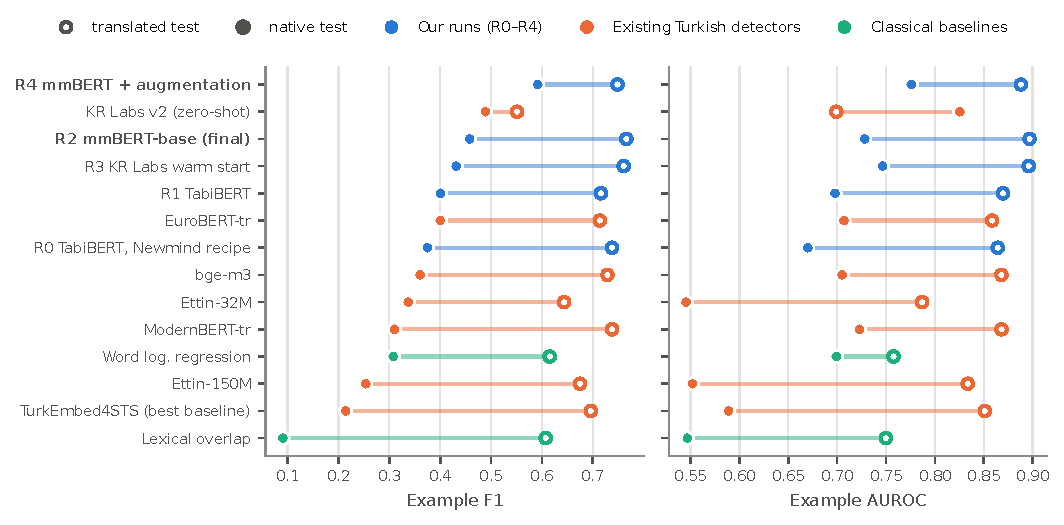
\includegraphics[width=\textwidth]{fig6_translated_vs_native.pdf}
\caption{Each system on the translated final test (open) and the native test (filled).}
\label{fig:native}
\end{figure*}

\section{Discussion and Limitations}
\textbf{The base model matters most.} TabiBERT tokenizes Turkish more efficiently, but mmBERT wins on this task. Possible reasons:
\begin{itemize}
\item the translated data keeps English structure;
\item 9\% of TabiBERT tokens straddle two words, which blurs span boundaries;
\item mmBERT is twice the size.
\end{itemize}

\textbf{Protocol drives conclusions.} Thresholds alone move some detectors by more than 0.2 example F1, and the best dev baseline regressed on test. Pre-registration and a single test pass keep the claims honest.

\textbf{Translated benchmarks overstate performance.} Ranking quality (AUROC) degrades less than F1, so part of the gap is calibration. Native training data closes the gap most.

\textbf{Limitations.}
\begin{itemize}
\item Training data and the main test are machine-translated.
\item The native set is small. Its labels are LLM-made with a 50-row human check that was not fully blind, and its spans were not edited by a human.
\item Its hallucinations come almost entirely from Qwen on rewritten questions.
\item R0 has one seed.
\item The data licenses are non-commercial.
\end{itemize}

\section{Conclusion}
Under one reproducible protocol, an mmBERT-base detector beats every existing Turkish detector on the translated test. A native Turkish test set shows that all detectors lose much of that performance on natural Turkish answers, and that native Turkish training data is the most promising remedy. Code, splits, labels and all result files are public in the project repository.

\begin{thebibliography}{99}
\bibitem{kovacs2025lettucedetect} Á. Kovács and G. Recski, ``LettuceDetect: A hallucination detection framework for RAG applications,'' arXiv:2502.17125, 2025.
\bibitem{tas2025turk} S. Taş, M. El Huseyni, Ö. Ezerceli, R. Bayraktar, and F. B. Terzioğlu, ``Turk-LettuceDetect: A hallucination detection models for Turkish RAG applications,'' arXiv:2509.17671, 2025.
\bibitem{niu2024ragtruth} C. Niu \emph{et al.}, ``RAGTruth: A hallucination corpus for developing trustworthy retrieval-augmented language models,'' in \emph{Proc. ACL}, 2024, pp. 10862--10878.
\bibitem{warner2024modernbert} B. Warner \emph{et al.}, ``Smarter, better, faster, longer: A modern bidirectional encoder for fast, memory efficient, and long context finetuning and inference,'' arXiv:2412.13663, 2024.
\bibitem{belyi2025luna} M. Belyi, R. Friel, S. Shao, and A. Sanyal, ``Luna: A lightweight evaluation model to catch language model hallucinations with high accuracy and low cost,'' in \emph{Proc. COLING: Industry Track}, 2025, pp. 398--409.
\bibitem{song2024raghat} J. Song \emph{et al.}, ``RAG-HAT: A hallucination-aware tuning pipeline for LLM in retrieval-augmented generation,'' in \emph{Proc. EMNLP: Industry Track}, 2024, pp. 1548--1558.
\bibitem{su2025rl4hs} H. Su \emph{et al.}, ``Learning to reason for hallucination span detection,'' arXiv:2510.02173, 2025.
\bibitem{dong2026sopo} J. Dong, Z. Bai, P. Zhu, and P. Zhou, ``SOPO: Socratic guided policy optimization for span-level hallucination detection,'' arXiv:2610.32212, 2026.
\bibitem{kovacs2026beyond} Á. Kovács \emph{et al.}, ``Beyond document grounding: Span-level hallucination detection over code, tool output, and documents,'' arXiv:2607.00895, 2026.
\bibitem{ogasa2025multiview} Y. Ogasa and Y. Arase, ``Hallucinated span detection with multi-view attention features,'' arXiv:2504.04335, 2025.
\bibitem{itkin2026temporal} I. Itkin, ``Temporal multi-signal fusion for token-level hallucination detection,'' arXiv:2608.18115, 2026.
\bibitem{kose2026ragturk} S. K. Köse \emph{et al.}, ``RAGTurk: Best practices for retrieval augmented generation in Turkish,'' in \emph{Proc. SIGTURK Workshop at EACL}, 2026, arXiv:2602.03652.
\bibitem{abdaljalil2026halluversem3} S. Abdaljalil, P. Sharma, E. Serpedin, and H. Kurban, ``Halluverse-M3: A multitask multilingual benchmark for hallucination in LLMs,'' arXiv:2602.06920, 2026.
\bibitem{abdaljalil2025halluverse25} S. Abdaljalil, H. Kurban, and E. Serpedin, ``HalluVerse25: Fine-grained multilingual benchmark dataset for LLM hallucinations,'' arXiv:2503.07833, 2025.
\bibitem{turker2025tabibert} M. Türker, A. E. Kızıloğlu, O. Güngör, and S. Üsküdarlı, ``TabiBERT: A large-scale ModernBERT foundation model and a unified benchmark for Turkish,'' arXiv:2512.23065, 2025.
\bibitem{marone2025mmbert} M. Marone, O. Weller, W. Fleshman, E. Yang, D. Lawrie, and B. Van Durme, ``mmBERT: A modern multilingual encoder with annealed language learning,'' arXiv:2509.06888, 2025.
\bibitem{boizard2025eurobert} N. Boizard \emph{et al.}, ``EuroBERT: Scaling multilingual encoders for European languages,'' arXiv:2503.05500, 2025.
\bibitem{weller2025ettin} O. Weller, K. Ricci, M. Marone, A. Chaffin, D. Lawrie, and B. Van Durme, ``Seq vs seq: An open suite of paired encoders and decoders,'' arXiv:2507.11412, 2025.
\bibitem{thoresen2026multiwiki} F. Thoresen and D. S. Smart, ``A multilingual hallucination benchmark: MultiWikiQHalluA,'' arXiv:2605.02504, 2026.
\bibitem{yang2025qwen3} A. Yang \emph{et al.}, ``Qwen3 technical report,'' arXiv:2505.09388, 2025.
\end{thebibliography}

\end{document}
